%!TEX TS-program = xelatex

% Шаблон документа LaTeX создан в 2018 году
% Алексеем Подчезерцевым
% В качестве исходных использованы шаблоны
% 	Данилом Фёдоровых (danil@fedorovykh.ru) 
%		https://www.writelatex.com/coursera/latex/5.2.2
%	LaTeX-шаблон для русской кандидатской диссертации и её автореферата.
%		https://github.com/AndreyAkinshin/Russian-Phd-LaTeX-Dissertation-Template

\documentclass[a4paper,14pt]{article}


%%% Работа с русским языком
\usepackage[english,russian]{babel}   %% загружает пакет многоязыковой вёрстки
\usepackage{fontspec}      %% подготавливает загрузку шрифтов Open Type, True Type и др.
\defaultfontfeatures{Ligatures={TeX},Renderer=Basic}  %% свойства шрифтов по умолчанию
\setmainfont[Ligatures={TeX,Historic}]{Times New Roman} %% задаёт основной шрифт документа
\setsansfont{Comic Sans MS}                    %% задаёт шрифт без засечек
\setmonofont{Courier New}
\usepackage{indentfirst}
\frenchspacing

\renewcommand{\epsilon}{\ensuremath{\varepsilon}}
\renewcommand{\phi}{\ensuremath{\varphi}}
\renewcommand{\kappa}{\ensuremath{\varkappa}}
\renewcommand{\le}{\ensuremath{\leqslant}}
\renewcommand{\leq}{\ensuremath{\leqslant}}
\renewcommand{\ge}{\ensuremath{\geqslant}}
\renewcommand{\geq}{\ensuremath{\geqslant}}
\renewcommand{\emptyset}{\varnothing}

%%% Дополнительная работа с математикой
\usepackage{amsmath,amsfonts,amssymb,amsthm,mathtools} % AMS
\usepackage{icomma} % "Умная" запятая: $0,2$ --- число, $0, 2$ --- перечисление

%% Номера формул
%\mathtoolsset{showonlyrefs=true} % Показывать номера только у тех формул, на которые есть \eqref{} в тексте.
%\usepackage{leqno} % Нумерация формул слева	

%% Перенос знаков в формулах (по Львовскому)
\newcommand*{\hm}[1]{#1\nobreak\discretionary{}
	{\hbox{$\mathsurround=0pt #1$}}{}}

%%% Работа с картинками
\usepackage{graphicx}  % Для вставки рисунков
\graphicspath{{images/}}  % папки с картинками
\setlength\fboxsep{3pt} % Отступ рамки \fbox{} от рисунка
\setlength\fboxrule{1pt} % Толщина линий рамки \fbox{}
\usepackage{wrapfig} % Обтекание рисунков текстом

%%% Работа с таблицами
\usepackage{array,tabularx,tabulary,booktabs} % Дополнительная работа с таблицами
\usepackage{longtable}  % Длинные таблицы
\usepackage{multirow} % Слияние строк в таблице
\usepackage{float}% http://ctan.org/pkg/float

%%% Программирование
\usepackage{etoolbox} % логические операторы


%%% Страница
\usepackage{extsizes} % Возможность сделать 14-й шрифт
\usepackage{geometry} % Простой способ задавать поля
\geometry{top=20mm}
\geometry{bottom=20mm}
\geometry{left=20mm}
\geometry{right=10mm}
%
%\usepackage{fancyhdr} % Колонтитулы
% 	\pagestyle{fancy}
%\renewcommand{\headrulewidth}{0pt}  % Толщина линейки, отчеркивающей верхний колонтитул
% 	\lfoot{Нижний левый}
% 	\rfoot{Нижний правый}
% 	\rhead{Верхний правый}
% 	\chead{Верхний в центре}
% 	\lhead{Верхний левый}
%	\cfoot{Нижний в центре} % По умолчанию здесь номер страницы

\usepackage{setspace} % Интерлиньяж
\onehalfspacing % Интерлиньяж 1.5
%\doublespacing % Интерлиньяж 2
%\singlespacing % Интерлиньяж 1

\usepackage{lastpage} % Узнать, сколько всего страниц в документе.

\usepackage{soul} % Модификаторы начертания

\usepackage{hyperref}
\usepackage[usenames,dvipsnames,svgnames,table,rgb]{xcolor}
\hypersetup{				% Гиперссылки
	unicode=true,           % русские буквы в раздела PDF
	pdftitle={Заголовок},   % Заголовок
	pdfauthor={Автор},      % Автор
	pdfsubject={Тема},      % Тема
	pdfcreator={Создатель}, % Создатель
	pdfproducer={Производитель}, % Производитель
	pdfkeywords={keyword1} {key2} {key3}, % Ключевые слова
	colorlinks=true,       	% false: ссылки в рамках; true: цветные ссылки
	linkcolor=black,          % внутренние ссылки
	citecolor=black,        % на библиографию
	filecolor=magenta,      % на файлы
	urlcolor=cyan           % на URL
}

\usepackage{csquotes} % Еще инструменты для ссылок

%\usepackage[style=authoryear,maxcitenames=2,backend=biber,sorting=nty]{biblatex}

\usepackage{multicol} % Несколько колонок

\usepackage{tikz} % Работа с графикой
\usepackage{pgfplots}
\usepackage{pgfplotstable}
\begin{document} % конец преамбулы, начало документа
\begin{titlepage}
	\begin{center}
		ФЕДЕРАЛЬНОЕ  ГОСУДАРСТВЕННОЕ АВТОНОМНОЕ \\
		ОБРАЗОВАТЕЛЬНОЕ УЧРЕЖДЕНИЕ ВЫСШЕГО ОБРАЗОВАНИЯ\\
		«НАЦИОНАЛЬНЫЙ ИССЛЕДОВАТЕЛЬСКИЙ УНИВЕРСИТЕТ\\
		«ВЫСШАЯ ШКОЛА ЭКОНОМИКИ»
	\end{center}
	
	\begin{center}
		\textbf{Московский институт электроники и математики}
	\end{center}
	\vspace{1ex}	
	\begin{center}
		Подчезерцев Алексей Евгеньевич, группа БИВ172
	\end{center}	
	\vspace{1ex}
	\begin{center}
		\textbf{КОМПЬЮТЕРНАЯ ИГРА «ЭРУДИТ» (SCRABBLE)}
	\end{center}	
	\vspace{2ex}
	\begin{center}
		Курсовая работа\\
		по направлению 09.03.01 Информатика и вычислительная техника\\
		студента образовательной программы бакалавриата\\
		«Информатика и вычислительная техника»
	\end{center}
	\vspace{2ex}
	\begin{flushright}
		Студент $\rule{5cm}{0.15mm}$ А.Е. Подчезерцев 
	\end{flushright}
	\vspace{3ex}
	\begin{flushright}
		Руководитель\\
		$\rule{5cm}{0.15mm}$ Е.А. Ерохина
	\end{flushright}
	\vfill
	\begin{center}
		Москва \the\year г.
	\end{center}
\end{titlepage}
\tableofcontents
\pagebreak
\section{Аннотация}
	Ежедневно люди проводят много времени пытаясь скрасить ожидание, например в транспорте.
	Игре <<Эрудит>> в этом году исполняется 50 лет.
	Данная игра расширяет кругозор и словарный запас человека.
	Кроме того, игра позволяет скоротать время в ожидании чего-либо, либо отдохнуть в компании друзей.
	Так же реализация данного проекта даст навыки командной работы, применения на практике различных алгоритмов.
	Поэтому мы выбрали данную тему для работы. В качестве результата разработки был получен программный продукт, реализующий методы, необходимые для данной игры.

\section*{Annotation}
Every day people spend a lot of time trying to brighten up the expectation, for example in transport.
The game <<Scrabble>> this year marks 50 years.
This game expands the horizons and vocabulary of a person.
In addition, allows you to pass the time waiting for something, or relax with friends.
In addition, this project will give us skills of teamwork, chance to make various algorithms in practice.
So, we chose this subject for work. As a result of the development was obtained a software product that implements the necessary methods for the game.

\pagebreak

\section{Введение}
	Наша курсовая работа посвящена разработке игры <<Эрудит>>.
	Суть игры заключается в том, что игрокам по очереди необходимо выставлять фишки на игровом поле так, чтобы любая последовательность букв образовывала слово.
	
	\subsection{Анализ готовых решений}
	Изначально <<Эрудит>> рассматривалась как настольная игра для нескольких человек, однако в эпоху информационных технологий были разработаны компьютерные варианты, которые позволяют играть нескольким игрокам, преимущественно по сети Интернет.
	Поэтому наше решение позволит играть одному игроку против компьютерных соперников.
	
	\subsection{Цель и задачи работы}
	\begin{itemize}
		\item \textbf{Разработать компьютерный вариант настольной игры <<Эрудит>>.}
		\item Создать возможность играть против одного или нескольких компьютерных соперников.
		\item Реализовать методы для хранения словаря, который можно расширять.
		\item Программа должна работать стабильно при всех возможных вариантах игры.
	\end{itemize}

	\subsection{Анализ используемых средств}
	В качестве основного языка программирования был выбран Python 3.
	Данный язык ускоряет процесс разработки, имеет дружелюбный синтаксис и богатую стандартную библиотеку, возможности которой можно легко расширить с помощью дополнительных пакетов.
	
	Так как наше приложение предполагает наличие пользовательского интерфейса, был подключен модуль $PyQt5$, который позволяет быстро и легко создавать пользовательские интерфейсы.
	
	Для взаимодействия команды разработчиков использовалась система контроля версий GIT с веб-сервисом GitHub.
	Данная комбинация позволяет работать над одним и тем же проектом команде разработчиков не уделяя много времени на решение вопросов, связанных с редактированием одинаковых файлов, конфликтов разных версий, обменом кодом посредством внешних носителей и другим схожим проблемам.
	
	Для проведения модульных тестов использовалась библиотека $unittest$, которая позволяет легко создать и выполнять тесты.
	
	В качестве среды программирования использовалась $IntelliJ IDEA$, благодаря которой можно работать с многими языками в одной среде, запускать отладку и проверять тесты.
	
	Данные программные средства существенно облегчили работу  и ускорили процесс разработки, что в итоге привело к созданию более мощного решения.
\section{Использованные классы}	
	\subsection{GameConfig}
	Информация о типах клеток на игровом поле, начальное число фишек у игроков, время хода, количество и цена каждой буквы и другие настройки хранятся в данном статичном классе.
	Это позволяет быстро изменить параметры игры.
	
	\subsection{Point}
	Данный класс содержит информацию о фишке на поле.
	Основных полей три - сама буква и её координаты на поле.
	По координатам определяется стоимость данной буквы и множитель очков слова.
	
	\subsection{Message}
	С помощью данного класса удобно передавать результат выполнения из функции.
	Логическая переменная сообщает программе итог работы, а сообщение выводится пользователю для информирования о событии.
	
	\subsection{MatrixResult}
	Класс-структура, хранящая результат обработки игрового поля и букв, которые необходимо на него поставить.
	Запоминает успех проверки, количество очков, найденные слова или слова с ошибкой, а так же сообщения об ошибке в случае провала.
		
	\subsection{GameDictionary}
	Это небольшой класс, однако он выполняет важные задачи.
	При его инициализации из файла загружаются словари слов русского языка и пользовательский.

	В качестве основы был взят толковый словарь русского языка.
	В процессе работы программы может быть вызван метод $append(self, item)$, который добавит в пользовательский словарь новое слово и сохранит его на диске.
	Кроме того, метод $prepare(self, alphabet)$ подготавливает словарь для компьютерного соперника.
	Это существенно облегчает работу алгоритма, так как сразу исключает те слова, которые никак не могут быть проставлены.
	
	\subsection{Matrix}
	В классе $Matrix$ осуществляется поиск слов и подсчет стоимости этих слов. Класс $Matrix$ содержит следующие методы: 
	
	\begin {itemize}
		\item$\_\_init\_\_$;
		\item $serch$;
		\item $\_prov$;
		\item $\_schit$;
		\item $reject\_temp$;	
		\item $pasteletters$;
		\item $\_ChekKoord$;
		\item $\_ValidationCheck$;
		\item $ValidationKoord$.
	\end {itemize}
	
	Инициализация переменных происходит в функции $\_\_init\_\_$.
	
	С основной задачей класса справляется функция $serch$.
	Для её работы нужны два массива: один с координатами новых точек, другой с новыми буквами.
	Но, перед тем как находить слова, необходимо подготовить и проверить матрицу и исходные массивы, за это отвечают функции $\_ChekKoord$, $pasteletters$ и $ValidationKoord$.
	
	$\_ChekKoord$ преобразует исходные массивы.
	Это делается из-за того, что в процессе составления массивов в них попадает ненужная информация.
	
	$pasteletters$ вставляет данные из массивов в матрицу.
	
	$ValidationKoord$ с помощью рекурсивной функции $\_ValidationCheck$ определяет правильность заполнения матрицы.
	Иными словами, функция проверяет выполнение следующих условий: конструкция из пересекающихся слов должна содержать в себе точку с координатами (7,7) и не должно быть букв, не принадлежащих этой конструкции.
	
	Функция $reject\_temp$ предназначена для работы с классом извне.
	Она очищает временные переменные.  
	
	Если $ValidationKoord$ возвращает положительный результат, можно начинать поиск слов.
	Пробегаемся по всей матрице (кроме последней строки и последнего столбца) и для каждой не пустой ячейки запускаем $\_prov$. $\_prov$ распознает начало слова, при положительном результате запускается функция $\_schit$. $\_schit$ проходит до конца слова, параллельно считая стоимость слова.
	Полученные результаты обрабатываются и передаются при помощи класса $MatrixResult$.
	
	\subsection{Player}
	Данный класс содержит базовую информацию об игроке: его имя, тип, номер, сложность (для компьютерного соперника) и др.
	Применяется на этапе подготовки игры, когда игроку не требуется какая-либо функциональность, но важно запомнить его статус.
	
	\subsection{TurnStruct}
	Специальная структура для хранения данных о ходе: ставит ли буквы игрок или же пропускает ход, какие буквы и куда помещает игрок, какие буквы будут сброшены, сколько очков можно получить за данное действие.
	
	\subsection[GamePlayer]{GamePlayer (наследуется от Player)}
	Данный абстрактный класс, кроме хранения информации об игроке, запоминает информацию о текущей игре.
	Содержит пустышки-методы, которые предупреждают игрока о начале его хода, о завершении хода противника, а так же следит за тем, не вышло ли время хода игрока. 
	Кроме того, в классе есть два метода, отвечающих за ход игрока - $check\_turn(self, turn)$ и $accept\_turn(self, turn)$. 
	Первый проверяет, можно ли выставить данным образом буквы. 
	В случае успеха возвращает найденные слова и очки, которые можно получить за ход. 
	Следующий метод применяет те действия, которые были переданы в данный метод, предварительно проверяя их. 
	Возвращает сообщение об успехе выполнения операции.
	
	\subsection[PlayerLocal]{PlayerLocal (наследуется от GamePlayer)}
	Данный класс предназначен для взаимодействия человека с интерфейсом игры.
	В нем переопределены методы, отвечающие за уведомление игрока о событиях.
	Они посылают специальный сигнал, с которым в дальнейшем работает пользовательский интерфейс, который в свою очередь отображает сообщение.
	
	\subsection[PlayerBot]{PlayerBot (наследуется от GamePlayer)}
	В данном классе реализованы все методы для взаимодействия компьютерного соперника с движком игры.
	При создании экземпляра данного класса дополнительно указывается сложность противника, а затем запускается новый поток, который отвечает за работу вычислительной части робота.
	Как только настанет ход компьютерного соперника, алгоритм начинает перебирать все возможные варианты слов и пытается вставить данное слово на игровое поле. 
	Для этого ищется соответствие каждой буквы на игровом поле. 
	При совпадении, отсутствии конфликтов перекрытия новым словом старого, наличии всех необходимых букв у игрока подсчитываются очки за такой теоретический ход.
	Действия продолжаются до тех пор, пока не закончатся слова или не останется слишком мало времени. 
	Затем все возможные варианты упорядочиваются по баллам, и выбирается тот, порядковый номер которого равен произведению длины массива на уровень сложности робота, после чего выбранный вариант применяется. 
	В случае отсутствия возможности сделать ход, компьютерный соперник пропускает ход, сбрасывая все буквы.
	
	\subsection{GameServer}
	Данный класс является ядром игры. 
	При инициализации обрабатывается массив игроков типа $Player$, которые затем преобразуются в дочерние классы класса $GamePlayer$, подготавливается алфавит, игровое поле, запускается новый поток, в котором будут проходить действия игры (дабы не блокировать основной). 
	Дополнительный поток на каждой итерации выполняет следующие действия:
	
	\begin {itemize}
		\item дает недостающие буквы игроку;
		\item приглашает его сделать ход;
		\item ожидает завершения;
		\item начисляет очки и бонусы;
		\item определяет, не завершился ли ход;	
		\item уведомляет всех о завершении хода.
	\end {itemize}

	
\section{Классы для работы с графическим интерфейсом}
Для работы с графическим интерфейсом было решено использовать библиотеку $PyQt5$. 
$PyQt5$ одна из самых мощных и популярных кросс-платформенных библиотек GUI.
	\subsection{Fishka}
	Класс $Fishka$ наследуется от класса $QPushButton$ из библиотеки $PyQt5$. 
	Новый класс необходим для упрощения работы с буквами, каждая кнопка, фишка, знает о себе всю необходимую информацию.
	\subsection{GameWindow}
	Данный класс предназначен для интерактивного взаимодействия с пользователем в процессе самой игры.
	
	Класс $GameWindow$ наследуется от класса из библиотеки $PyQt$ $QWidget$.	
	Функция $\_\_init\_\_$  инициализирует переменные, вычисляет размеры и создает окно.	
	Далее происходит отрисовка фона.
	Результат работы предоставлен на \imref{img:background}
	Выполняют функции $paintEvent$ и $drawBackground$.
	\begin{figure}[H]
		\centering
		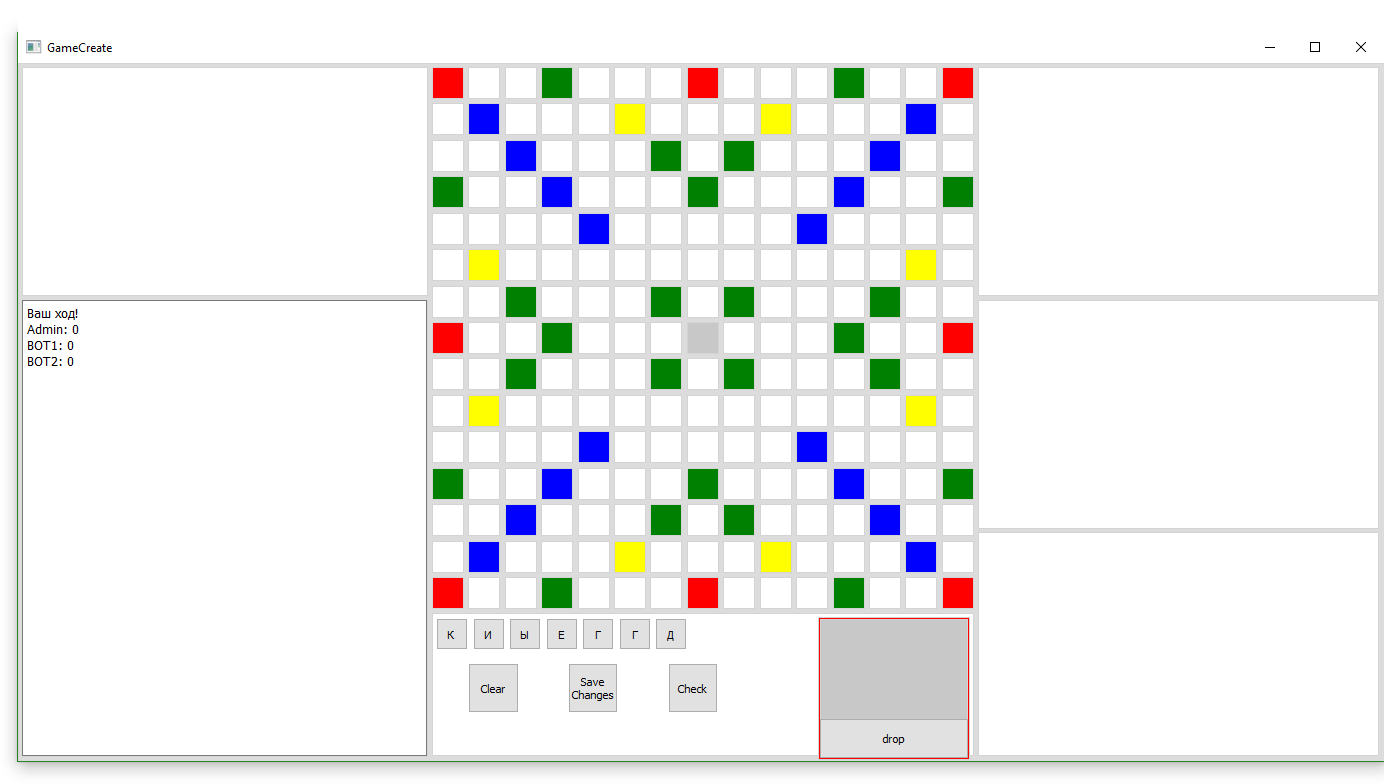
\includegraphics[width=\linewidth]{bigpole.png}
		\caption{Задний фон}
		\label{img:background}
	\end{figure}
	
	% TODO	
	В функции $initUI$ создаются виджеты кнопок (QPushButton) и виджет изменения строки (QLineEdet), который будет использоваться в качестве консоли.
		
	% TODO
	После ввода текста в консоль и нажатия кнопки "Enter"\ вызывается функция $enter$.
	В зависимости от введенного текста могут выполниться следующие функции: $Help$, $ProverkaKoordinat$,  $lastLetters$,  $ClearChanges$, $SeveChangesForm$, $dobavlenie$, $Drop$.
	
	% TODO
	\begin {itemize}
	\item $Help$ (Help()) - показывает все возможные команды, которые можно выполнить используя консоль
	\item $ProverkaKoordinat$ (ProverkaKoordinat(i, x, y)) - переносит букву с номером i на позицию (x, y), формирует массивы с новыми буквами и их координатами	
	\item $lastLetters$ (lastLetters()) - отрисовывает буквы, которые вносились в матрицу ранее.
	\item $ClearChanges$ (ClearChanges()) - очищает временные переменные, возвращает на места буквы, переставленные на этом ходу.
	\item $SeveChangesForm$ (SeveChangesForm()) - отправляет данные на проверку.
	\item $dobavlenie$ (dobavlenie(words)) - с разрешения пользователя добавляет новые слова в словарь. Пример такого уведомления изображен на \imref{img:dob}.
	\begin{figure}[bhtp]
		\centering
		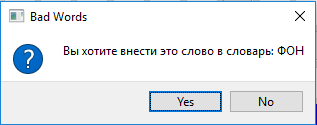
\includegraphics[width=0.3\linewidth]{dobavlenie.png}
		\caption{запрос на добавление нового слова}
		\label{img:dob}
	\end{figure}
	\item $Drop$ (Drop(dr)) - сбрасывает буквы, номера которых находятся в массиве dr.
	\end {itemize}
	
	Для вывода уведомлений пользователю использовалась функция $add\_to\_console$, коротая добавляла текст уведомления о событиях в игре, а так же сообщала количество баллов каждого игрока (\imref{img:game}).

	\begin{figure}[H]
		\centering
		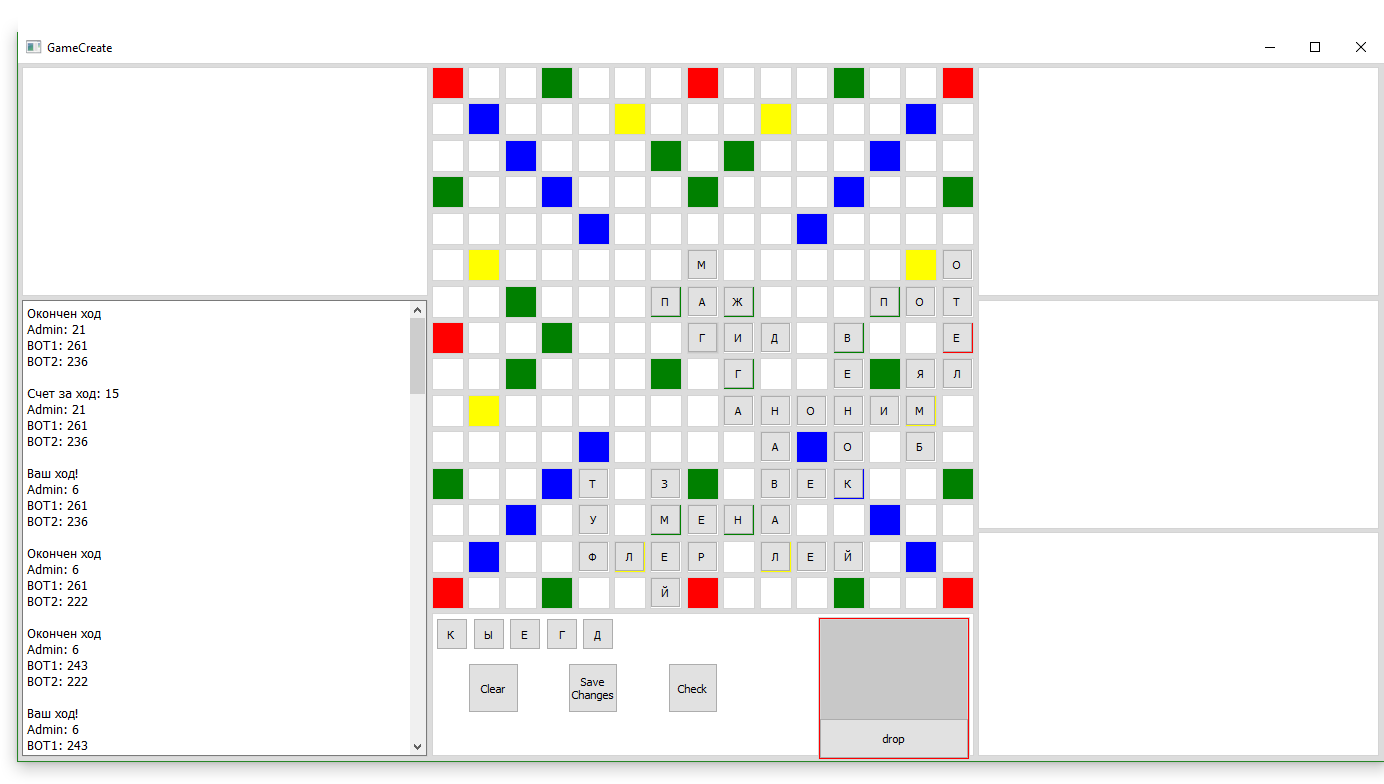
\includegraphics[width=\linewidth]{game.png}
		\caption{Игровое поле после нескольких ходов}
		\label{img:game}
	\end{figure}

\section{Процесс работы программы}
	В данный момент работа программы начинается с запуска стартовой формы (\imref{img:start}).
	Пользователь выбирает количество компьютерных соперников, с которыми он будет играть, а так же их уровень сложности от 0 до 1.
	При нажатии кнопки <<Запустить>> создается игровая форма, игровой сервер, интерфейсы взаимодействия локального игрока и компьютерных соперников, загружается словарь и подготавливается алфавит, после чего готовая форма отображается пользователю.

	\begin{figure}[H]
		\centering
		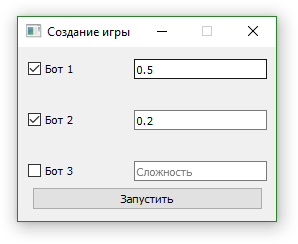
\includegraphics[width=0.4\linewidth]{start.png}
		\caption{Форма создания игры}
		\label{img:start}
	\end{figure}

	\subsection[Отрисовка интерфейса]{Отрисовка пользовательского интерфейса}
	Отрисовка интерфейса начинается с создания формы, где задаются ее размеры, а также местоположение на экране.
	Далее начинается отрисовка заднего фона и игрового поля, при этом местоположение каждого элемента на поле запоминается.
		
	\subsection{Игровая механика}
	Игроки ходят по очереди, действия компьютерного соперника выполняются автоматически, без вмешательства пользователя.
	Человеку предоставлена возможность передавать команды через интуитивный графический интерфейс.
	С его помощью можно фишки установить на поле или сбросить некоторое число, проверить правильность хода, добавить новые слова, отменить все свои действия.
	Затем программа проверяет действия пользователя, и если она не нашла некоторые слова в своем словаре, то спрашивает игрока является ли найденная последовательность букв словом.
	В случае успеха действия игрока запоминаются и ход передается следующему.
	После каждого хода показывается уведомление, а также при наступлении очереди текущего игрока. На \imref{img:game} показан промежуточный этап игры.
	
	\subsection{Завершение игры}
	При достижении условий окончания игры - закончились фишки или все игроки пропустили ход определенное число раз - сервер завершает свою работу и показывает сообщение о баллах, которые набрал каждый игрок (\imref{img:endGame}).
	
	\begin{figure}[bhtp]
		\centering
		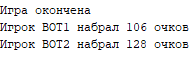
\includegraphics{gameresult.png}
		\caption{Итог игры}\label{img:gameresult}
		\label{img:endGame}
	\end{figure}
\section{Тестирование}
	Процесс разработки большого коллективного проекта достаточно сложный.
	Легко допустить ошибку, найти причину которой, а порой и заметить эффект, достаточно сложно. Поэтому были созданы специальные модульные тесты, проверяющие работу некоторых функций, тестировать которые вручную было бы утомительно.
	
	\subsection{Словарь}
	Был подготовлен небольшой словарь, выборку из которого случайным образом не сложно произвести один раз вручную.
	Затем на ее основе были созданы данные тесты
	
	Список слов: биосфера, блюз, дворянство, домолачивание, заковывание, изъян, киноведение, колеровщик, координированность, митраизм, налавливание, неминуемость, одухотворенность, окраина, плавсостав, поборник, подхват, приматывание, пролысина, сипловатость, солододробилка, топаз, трином, трехсотлетие, умывание, хранилище, централизация, шейх.
	\begin{table}[!h]
		\begin{center}
		\begin{flushleft}
			\tablecaption{Тестирование словаря}			
		\end{flushleft}
		
		\begin{tabular}{|c|c|}
			\hline
			         Входные данные          & Контрольное значение \\ \hline
			АБВГДЕЖЗИЙКЛМНОПРСТУФХЦЧШЩЪЫЬЭЮЯ &    Длина словаря     \\ \hline
			               А                 &          0           \\ \hline
			              БЛЮЗ               &          1           \\ \hline
			АБВГДЕЖЗИЙКЛМНОПРСТУФХЦЧШЩЪЫЬЭЮ  &  Длина словаря - 3   \\ \hline
		\end{tabular}
		\end{center}
	\end{table}

	\subsection{Фишка}
	Постановку точки на поле так же легко проверить.
	Для этого сравнивалось контрольное значение типа точки с тем, которое она получила при инициализации.
	На вход подается координаты и буква, на выходе закодированный номер типа.
	
	\begin{table}[!h]
		\begin{center}
			\tablecaption{Тестирование фишки на игровом поле}
			\begin{tabular}{|c|c|}
				\hline
				Входные данные          & Контрольное значение \\ \hline
				0 0 Я& 4 \\ \hline
				6 8 Я& 1 \\ \hline
				4 4 Я& 2 \\ \hline
				1 5 Я& 3 \\ \hline
				1 2 Я& 0 \\ \hline
			\end{tabular}
		\end{center}
	\end{table}

	\subsection{Компьютерный противник}
	При разработке алгоритмов робота часто возникали проблемы, при котором компьютер решал задачу слишком долго или вовсе не находил решение.
	Полностью проверить ход на верность затруднительно, однако можно легко узнать, выполняет какие-либо действия алгоритм или нет.
	Для этого были созданы 2 робота, играющие друг против друга.
	Успехом считалось, что каждый робот наберет некоторое число очков за небольшое время после старта.
	
	\subsection{Обработка результатов}
	\begin{figure}[bhtp]
		\centering		
		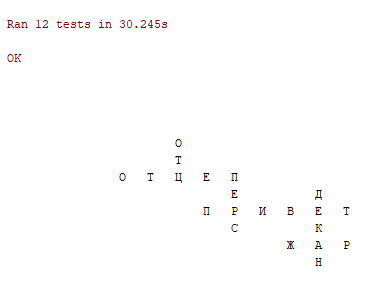
\includegraphics[scale=0.8]{unittests.png}
		\caption{Результат модульного тестирования}\label{img:tests}
	\end{figure}
	
	На \imref{img:tests} показан результат успешного тестирования.
	Нет ни одного слова с ошибкой, показано игровое поле, которое заполнили два компьютерных соперника, играющие друг против друга.
	
	Однако, это не единственный этап тестирования.
	В случае успеха на данном этапе выполняется ручное тестирование.
	Программа должна запуститься, успешно и правильно обрабатывать команды пользователя, выводить результат, компьютерный соперник должен совершать некоторые ходы.
	
\section{Вывод}
	Мы добились поставленной цели.
	У нас есть компьютерная версия игры <<Эрудит>>, в которой можно играть против нескольких компьютерных соперников.
	В игре есть возможность добавление новых слов в словарь.
	В ходе многочисленных тестов программа работала стабильно.
	
\newpage 
\renewcommand{\refname}{{\normalsize СПИСОК ИСПОЛЬЗОВАННЫХ ИСТОЧНИКОВ}} 
\centering 
\begin{thebibliography}{9} 
	\addcontentsline{toc}{section}{\refname} 
	\bibitem{python} Доусон М. Программируем на Python //СПб.: Питер. – 2014. – Т. 416.
	\bibitem{pyqt} Прохоренок Н. А. Python 3 и PyQt. Разработка приложений. – БХВ-Петербург, 2012.
	\bibitem{scrabble} Скрэббл, URL: \url{https://ru.wikipedia.org/wiki/Скрэббл} (дата обращения 13.01.2018) 
	
\end{thebibliography}
\end{document} % конец документа

